\documentclass[12pt,a4paper]{article}
\usepackage[utf8]{vietnam}
\usepackage{amsmath,amssymb,amsfonts,mathrsfs}
\usepackage[left=1.5cm,right=1.5cm,top=2cm,bottom=2cm,headheight=17pt]{geometry}
\usepackage{enumitem}
\usepackage{array}
\usepackage{graphicx}
\usepackage{tikz}
\usetikzlibrary{arrows.meta,calc,patterns}
\usepackage{fancyhdr}

\pagestyle{fancy}
\fancyhf{}
\lhead{\small\textbf{HƯỚNG TỚI THPTQG 2027}}
\rhead{\small\textit{Người biên soạn: Dương Gia Bảo}}
\rfoot{\small Trang \thepage}
\renewcommand{\headrulewidth}{0.4pt}

\begin{document}

\noindent
\begin{minipage}[t]{0.40\textwidth}
    \centering
    \textbf{HƯỚNG TỚI THPTQG 2027}\\[-2pt]
    \rule{3.2cm}{0.6pt}\\[4pt]
    \textbf{ĐỀ CHÍNH THỨC}
\end{minipage}\hfill
\begin{minipage}[t]{0.58\textwidth}
    \centering
    \textbf{ĐỀ THI KHẢO SÁT CHẤT LƯỢNG}\\
    \textbf{ĐỀ SỐ 7}\\
    \textbf{Môn thi: TOÁN}\\
    \textit{\small Thời gian làm bài: 90 phút, không kể thời gian phát đề}
\end{minipage}

\vspace{0.2cm}
\noindent
\begin{minipage}[b]{0.78\textwidth}
    \textbf{Họ và tên:}\dotfill\textbf{SBD:}\makebox[3.5cm]{\dotfill}
\end{minipage}\hfill
\begin{minipage}[b]{0.20\textwidth}
    \hfill
    \setlength{\fboxrule}{0.8pt}%
    \fbox{\begin{minipage}{2.3cm}
        \centering
        \textbf{\small Mã đề thi}\\
        \textbf{0007}
    \end{minipage}}
\end{minipage}
\vspace{0.2cm}

% ==========================================
% PHẦN I
% ==========================================
\section*{\large PHẦN I. CÂU TRẮC NGHIỆM NHIỀU PHƯƠNG ÁN LỰA CHỌN}
\textit{Thí sinh trả lời từ câu 1 đến câu 12. Mỗi câu hỏi thí sinh chỉ chọn một phương án. Mỗi câu trả lời đúng được 0,25 điểm.}

\begin{enumerate}[label=\textbf{Câu \arabic*:}, leftmargin=*]

\item Cho hàm số $y = \dfrac{x^2 - 2mx + m^2 + m - 2}{x - m}$. Có bao nhiêu giá trị nguyên của tham số $m \in [-10; 10]$ để đồ thị hàm số có hai điểm cực trị $A, B$ sao cho độ dài đoạn thẳng $AB$ không vượt quá $2\sqrt{15}$?
\begin{enumerate}[label=\Alph*.]
    \item $3$.
    \item $4$.
    \item $2$.
    \item $5$.
\end{enumerate}

\item Số nghiệm nguyên của bất phương trình $\log_2(x - 1) + \log_2(9 - x) \ge 3$ là
\begin{enumerate}[label=\Alph*.]
    \item $6$.
    \item $4$.
    \item $5$.
    \item $7$.
\end{enumerate}

\item Cho hàm số $y = f(x)$ có đạo hàm liên tục trên $\mathbb{R}$ và thỏa mãn $f(x) + x f'(x) = 4x^3 - 6x^2 + 2x + 1$ với mọi $x \in \mathbb{R}$. Giá trị của tích phân $I = \int_0^2 f(x)\,\mathrm{d}x$ bằng
\begin{enumerate}[label=\Alph*.]
    \item $\dfrac{10}{3}$.
    \item $4$.
    \item $\dfrac{14}{3}$.
    \item $\dfrac{8}{3}$.
\end{enumerate}

\item Trong không gian $Oxyz$, cho mặt phẳng $(P): x - y - 2z + 4 = 0$ và đường thẳng $\Delta: \dfrac{x - 4}{2} = \dfrac{y + 2}{-1} = \dfrac{z - 4}{1}$. Đường thẳng $d$ đi qua điểm $A(2; -1; 3)$, cắt mặt phẳng $(P)$ và đường thẳng $\Delta$ lần lượt tại $M, N$ sao cho $N$ là trung điểm của đoạn thẳng $AM$. Một vectơ chỉ phương của đường thẳng $d$ là
\begin{enumerate}[label=\Alph*.]
    \item $\vec{u}_1 = (1; -2; 2)$.
    \item $\vec{u}_2 = (2; -1; 1)$.
    \item $\vec{u}_3 = (1; -1; -2)$.
    \item $\vec{u}_4 = (2; 1; -1)$.
\end{enumerate}

\item Bạn An đi học mỗi ngày bằng một trong hai phương tiện: xe buýt hoặc xe đạp điện. Xác suất An chọn đi xe buýt là $0{,}40$ và chọn đi xe đạp điện là $0{,}60$. Nếu An đi xe buýt thì xác suất bị muộn học là $0{,}06$; nếu An đi xe đạp điện thì xác suất bị muộn học là $0{,}02$. Biết rằng sáng thứ Hai bạn An bị muộn học, xác suất để sáng hôm đó An đã đi bằng xe buýt bằng
\begin{enumerate}[label=\Alph*.]
    \item $\dfrac{2}{3}$.
    \item $\dfrac{1}{3}$.
    \item $\dfrac{3}{4}$.
    \item $\dfrac{2}{5}$.
\end{enumerate}

\item Cân nặng của $40$ quả mít trong một khu vườn được thống kê ở bảng tần số ghép nhóm sau:
\begin{center}
\begin{tabular}{|c|c|c|c|c|c|}
\hline
\textbf{Cân nặng (kg)} & $[4; 6)$ & $[6; 8)$ & $[8; 10)$ & $[10; 12)$ & $[12; 14)$ \\ \hline
\textbf{Số quả mít} & $6$ & $12$ & $10$ & $8$ & $4$ \\ \hline
\end{tabular}
\end{center}
Phương sai $s^2$ của mẫu số liệu ghép nhóm trên bằng
\begin{enumerate}[label=\Alph*.]
    \item $5{,}64$.
    \item $2{,}42$.
    \item $5{,}84$.
    \item $6{,}12$.
\end{enumerate}

\item Cho hàm số $f(x) = (x^2 - 5x + 7)e^x$. Giá trị lớn nhất của hàm số đã cho trên đoạn $[0; 3]$ bằng
\begin{enumerate}[label=\Alph*.]
    \item $3e$.
    \item $e^3$.
    \item $7$.
    \item $e^2$.
\end{enumerate}

\item Diện tích hình phẳng giới hạn bởi parabol $(P): y = x^2 - 4x + 3$ và đường thẳng $d: y = x - 1$ bằng
\begin{enumerate}[label=\Alph*.]
    \item $\dfrac{7}{2}$.
    \item $\dfrac{11}{3}$.
    \item $\dfrac{15}{4}$.
    \item $\dfrac{9}{2}$.
\end{enumerate}

\item Trong không gian $Oxyz$, cho mặt phẳng $(P): 2x - y + 2z - 16 = 0$ và hai điểm $A(1; 2; 1)$, $B(4; -1; 4)$. Gọi $M(a; b; c)$ là điểm thuộc mặt phẳng $(P)$ sao cho biểu thức $T = 2MA^2 + MB^2$ đạt giá trị nhỏ nhất. Giá trị của tổng $a + b + c$ bằng
\begin{enumerate}[label=\Alph*.]
    \item $8$.
    \item $5$.
    \item $6$.
    \item $9$.
\end{enumerate}

\item Cho cấp số cộng $(u_n)$ có công sai $d > 0$ thỏa mãn $u_2 + u_5 = 24$ và $u_3 \cdot u_4 = 135$. Tổng $10$ số hạng đầu tiên $S_{10}$ của cấp số cộng bằng
\begin{enumerate}[label=\Alph*.]
    \item $210$.
    \item $270$.
    \item $240$.
    \item $195$.
\end{enumerate}

\item Trong không gian $Oxyz$, cho tứ diện $ABCD$ với $A(2; -1; 1)$, $B(4; 3; -1)$, $C(1; 2; 4)$ và $D(5; 4; 6)$. Gọi $P, Q$ lần lượt là trung điểm của hai cạnh $AB$ và $CD$. Độ dài đoạn thẳng $PQ$ bằng
\begin{enumerate}[label=\Alph*.]
    \item $\sqrt{21}$.
    \item $\sqrt{29}$.
    \item $5$.
    \item $\sqrt{33}$.
\end{enumerate}

\item Một đội thanh niên tình nguyện gồm $6$ học sinh khối 12, $5$ học sinh khối 11 và $4$ học sinh khối 10. Chọn ngẫu nhiên đồng thời $4$ học sinh từ đội đi làm nhiệm vụ. Xác suất để $4$ học sinh được chọn có đủ cả $3$ khối và số học sinh khối 12 nhiều hơn số học sinh khối 10 bằng
\begin{enumerate}[label=\Alph*.]
    \item $\dfrac{40}{91}$.
    \item $\dfrac{15}{91}$.
    \item $\dfrac{30}{91}$.
    \item $\dfrac{20}{91}$.
\end{enumerate}

\end{enumerate}

% ==========================================
% PHẦN II
% ==========================================
\section*{\large PHẦN II. CÂU TRẮC NGHIỆM ĐÚNG/SAI}
\textit{Thí sinh trả lời từ câu 1 đến câu 4. Trong mỗi ý a), b), c), d) ở mỗi câu, thí sinh chọn Đúng hoặc Sai.}

\begin{enumerate}[label=\textbf{Câu \arabic*:}, leftmargin=*]

\item Một doanh nghiệp sản xuất và phân phối một dòng thiết bị cảm biến công nghiệp. Khi doanh nghiệp cung ứng $x$ ngàn thiết bị ra thị trường trong một quý ($x > 0$), giá bán của mỗi ngàn thiết bị được mô hình hóa bởi hàm cầu $p(x) = -x^2 + 9x + 120$ (triệu đồng/ngàn thiết bị). Tổng chi phí sản xuất và vận hành cho $x$ ngàn thiết bị là $C(x) = 72x + 100$ (triệu đồng). Gọi $R(x) = x \cdot p(x)$ là hàm tổng doanh thu và $L(x) = R(x) - C(x)$ là hàm tổng lợi nhuận ròng của doanh nghiệp (đơn vị: triệu đồng).
\begin{enumerate}[label=\alph*)]
    \item Hàm tổng doanh thu của doanh nghiệp là $R(x) = -x^3 + 9x^2 + 120x$ (triệu đồng).
    \item Hàm lợi nhuận ròng của doanh nghiệp là $L(x) = -x^3 + 9x^2 + 48x - 100$ (triệu đồng) và có đạo hàm $L'(x) = -3x^2 + 18x + 48$.
    \item Khi không bị giới hạn công suất nhà máy, doanh nghiệp đạt lợi nhuận ròng lớn nhất tại mức sản lượng $x = 6$ ngàn thiết bị.
    \item Nếu dây chuyền của nhà máy bị giới hạn công suất tối đa $x \le 6$ ngàn thiết bị mỗi quý thì mức lợi nhuận ròng lớn nhất doanh nghiệp có thể thu được là $296$ triệu đồng.
\end{enumerate}

\item Một trường THPT tiến hành khảo sát ngẫu nhiên $600$ học sinh khối 12 về sự yêu thích môn Toán và kết quả học tập môn Toán. Số liệu thống kê thu được như sau: có $400$ học sinh trả lời ``Thích học Toán'' và $200$ học sinh trả lời ``Không thích học Toán''. Thực tế kiểm tra cho thấy tỉ lệ học sinh đạt danh hiệu ``Giỏi Toán'' trong nhóm trả lời ``Thích học Toán'' là $75\%$, còn trong nhóm trả lời ``Không thích học Toán'' là $15\%$. Chọn ngẫu nhiên một học sinh trong $600$ học sinh được khảo sát. Gọi $T$ là biến cố ``Học sinh được chọn trả lời Thích học Toán'' và $G$ là biến cố ``Học sinh được chọn đạt danh hiệu Giỏi Toán''.
\begin{enumerate}[label=\alph*)]
    \item Xác suất của biến cố $T$ là $P(T) = \dfrac{2}{3}$ và xác suất của biến cố đối $\overline{T}$ là $P(\overline{T}) = \dfrac{1}{3}$.
    \item Xác suất có điều kiện để một học sinh đạt danh hiệu ``Giỏi Toán'' biết rằng học sinh đó trả lời ``Không thích học Toán'' là $P(G \mid \overline{T}) = 0{,}25$.
    \item Xác suất để một học sinh được chọn ngẫu nhiên trong đợt khảo sát đạt danh hiệu ``Giỏi Toán'' là $P(G) = 0{,}55$.
    \item Biết rằng học sinh được chọn đạt danh hiệu ``Giỏi Toán'', xác suất để học sinh đó đã trả lời ``Thích học Toán'' bằng $\dfrac{10}{11} \approx 90{,}91\%$.
\end{enumerate}

\item Trong vật lý âm học, mức cường độ âm $L$ (đơn vị: $\text{dB}$) tại một điểm được xác định bởi công thức $L = 10\log_{10}\!\left(\dfrac{I}{I_0}\right)$, trong đó $I$ (đơn vị: $\text{W/m}^2$) là cường độ âm tại điểm đó và $I_0 = 10^{-12}\text{ W/m}^2$ là cường độ âm chuẩn. Một kỹ thuật viên âm thanh đứng cố định tại vị trí $M$ giữa hai loa phát thanh $A$ và $B$. Khi chỉ bật riêng loa $A$, người đó đo được mức cường độ âm tại $M$ là $L_A = 80\text{ dB}$. Khi chỉ bật riêng loa $B$, người đó đo được mức cường độ âm tại $M$ là $L_B = 90\text{ dB}$. Biết rằng khi bật đồng thời cả hai loa thì cường độ âm tổng hợp tác động vào tai người tại $M$ bằng tổng cường độ âm của hai loa ($I = I_A + I_B$).
\begin{enumerate}[label=\alph*)]
    \item Cường độ âm do riêng loa $A$ gây ra tại vị trí $M$ là $I_A = 10^{-4}\text{ W/m}^2$.
    \item Cường độ âm do riêng loa $B$ gây ra tại vị trí $M$ là $I_B = 10^{-3}\text{ W/m}^2$, gấp $10$ lần cường độ âm của loa $A$.
    \item Khi bật đồng thời cả hai loa $A$ và $B$, mức cường độ âm tổng hợp mà kỹ thuật viên đo được tại $M$ bằng $L = L_A + L_B = 170\text{ dB}$.
    \item Thực tế khi bật đồng thời cả hai loa, mức cường độ âm tại vị trí $M$ xấp xỉ bằng $90{,}41\text{ dB}$ (làm tròn kết quả đến hàng phần trăm).
\end{enumerate}

\item \begin{minipage}[t]{0.55\linewidth}
Trong không gian $Oxyz$ (đơn vị trên mỗi trục tọa độ là kilômét), mặt phẳng $(Oxy)$ trùng với mặt đất và trục $Oz$ hướng thẳng đứng lên cao. Một khinh khí cầu nghiên cứu khí tượng đang bay ở độ cao ổn định $5\text{ km}$ so với mặt đất (tức cao độ $z_M = 5$). Tại thời điểm quan sát, thiết bị định vị trên khinh khí cầu $M(x; y; 5)$ nhận được tín hiệu đồng thời từ ba vệ tinh tại các vị trí $A(1; 1; 5)$, $B(4; 11; 13)$ và $C(16; 5; 10)$. Từ thời gian truyền sóng, hệ thống đo được khoảng cách từ khinh khí cầu $M$ đến ba vệ tinh lần lượt là $MA = 5\text{ km}$, $MB = 10\text{ km}$ và $MC = 13\text{ km}$.
\begin{enumerate}[label=\alph*)]
    \item Khoảng cách giữa hai vệ tinh $A$ và $B$ bằng $\sqrt{173}\text{ km}$.
    \item Vì khinh khí cầu ở độ cao $z_M = 5\text{ km}$ và cách vệ tinh $A(1; 1; 5)$ một khoảng bằng $5\text{ km}$ nên hoành độ $x$ và tung độ $y$ của khinh khí cầu thỏa mãn phương trình $(x - 1)^2 + (y - 1)^2 = 5$.
    \item Tọa độ vị trí chính xác của khinh khí cầu tại thời điểm quan sát là $M(4; 5; 5)$.
    \item Khoảng cách từ khinh khí cầu $M$ đến trạm điều khiển đặt tại gốc tọa độ $O(0; 0; 0)$ bằng $\sqrt{66} \approx 8{,}12\text{ km}$.
\end{enumerate}
\end{minipage}\hfill
\begin{minipage}[t]{0.42\linewidth}
\vspace{-0.4\baselineskip}
\centering
\resizebox{\linewidth}{!}{%
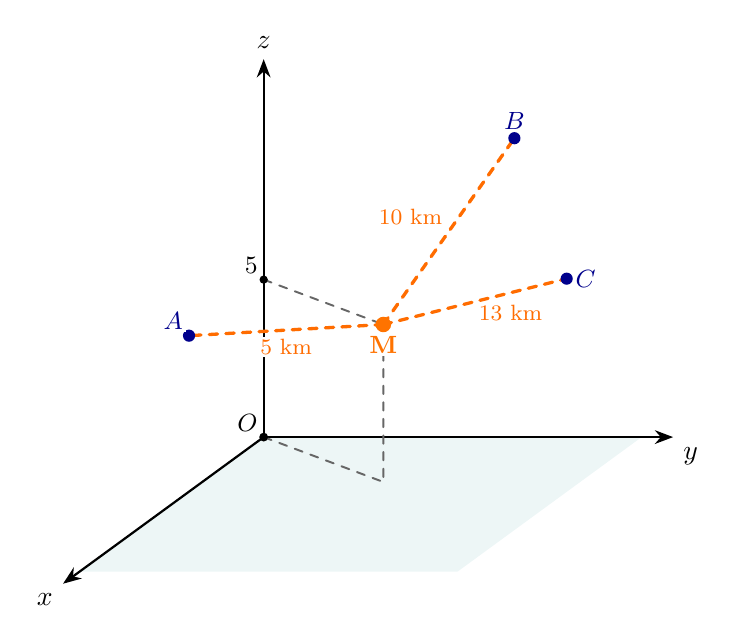
\begin{tikzpicture}[>=Stealth, line join=round, line cap=round,
    x={(-0.52cm,-0.38cm)}, y={(1cm,0cm)}, z={(0cm,1cm)}]
    \coordinate (O) at (0,0,0);
    \coordinate (M) at (1.5,2.3,2.0);
    \coordinate (Mxy) at (1.5,2.3,0);
    \coordinate (Oz5) at (0,0,2.0);
    \coordinate (A) at (2.4,0.3,2.2);
    \coordinate (B) at (0.8,3.6,4.1);
    \coordinate (C) at (2.6,5.2,3.0);

    % Mat dat Oxy
    \fill[teal!10, opacity=0.7] (0,0,0) -- (4.5,0,0) -- (4.5,4.8,0) -- (0,4.8,0) -- cycle;

    % 3 truc toa do Oxyz chuan SGK
    \draw[->, thick, black] (O) -- (4.9,0,0) node[below left] {$x$};
    \draw[->, thick, black] (O) -- (0,5.2,0) node[below right] {$y$};
    \draw[->, thick, black] (O) -- (0,0,4.8) node[above] {$z$};

    % Duong giong do cao z = 5
    \draw[dashed, black!60, line width=0.7pt] (O) -- (Mxy) -- (M);
    \draw[dashed, black!60, line width=0.7pt] (Oz5) -- (M);
    \fill[black] (Oz5) circle (1.5pt) node[above left=1pt, fill=white, inner sep=1pt] {\small $5$};

    % Tia tin hieu tu 3 ve tinh A, B, C den M
    \draw[dashed, very thick, orange!85!red] (M) -- (A) node[midway, below=2pt, fill=white, inner sep=0.8pt] {\footnotesize $5\text{ km}$};
    \draw[dashed, very thick, orange!85!red] (M) -- (B) node[midway, above left=1pt, fill=white, inner sep=0.8pt] {\footnotesize $10\text{ km}$};
    \draw[dashed, very thick, orange!85!red] (M) -- (C) node[midway, below right=0pt, fill=white, inner sep=0.8pt] {\footnotesize $13\text{ km}$};

    % Chi ghi ten diem A, B, C, M, O ngan gon
    \fill[black] (O) circle (1.6pt) node[above left=1pt, fill=white, inner sep=1pt] {\small $O$};
    \fill[blue!55!black] (A) circle (2.2pt) node[above left=1pt, fill=white, inner sep=1pt] {\small $A$};
    \fill[blue!55!black] (B) circle (2.2pt) node[above=2pt, fill=white, inner sep=1pt] {\small $B$};
    \fill[blue!55!black] (C) circle (2.2pt) node[right=2pt, fill=white, inner sep=1pt] {\small $C$};
    \fill[orange!90!red] (M) circle (2.8pt) node[below=3pt, fill=white, inner sep=1pt] {\small $\mathbf{M}$};
\end{tikzpicture}%
}
\end{minipage}

\end{enumerate}

% ==========================================
% PHẦN III
% ==========================================
\section*{\large PHẦN III. CÂU TRẮC NGHIỆM TRẢ LỜI NGẮN}
\textit{Thí sinh trả lời từ câu 1 đến câu 6. Điền đáp số theo quy chuẩn làm tròn được nêu trong từng câu.}

\begin{enumerate}[label=\textbf{Câu \arabic*:}, leftmargin=*]

\item \begin{minipage}[t]{0.55\linewidth}
Một cái hồ lớn có hai bờ $AB$ và $AC$ vuông góc với nhau tại góc hồ $A$. Tại một vị trí $K$ trong góc hồ cách bờ $AB$ một khoảng $1\text{ m}$ và cách bờ $AC$ một khoảng $8\text{ m}$, người ta đóng một chiếc cọc cố định, rồi dùng một cây sào thẳng $PQ$ ($P \in AB$, $Q \in AC$) tựa vào cọc $K$ để ngăn một góc tam giác $APQ$ thả bèo (bỏ qua đường kính của cọc và sào). Tính chiều dài ngắn nhất của cây sào $PQ$ theo đơn vị mét (làm tròn kết quả đến hàng phần trăm).
\end{minipage}\hfill
\begin{minipage}[t]{0.42\linewidth}
\vspace{-0.4\baselineskip}
\centering
\resizebox{\linewidth}{!}{%
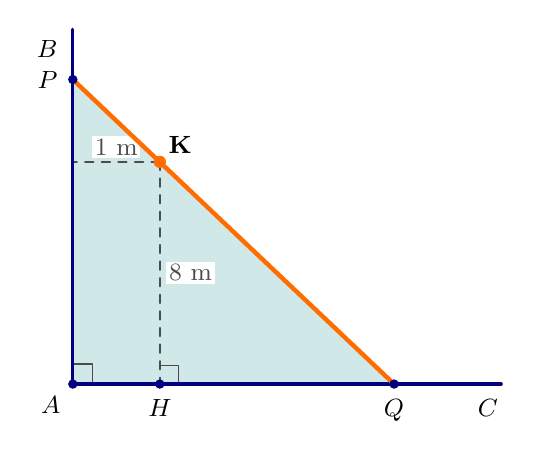
\begin{tikzpicture}[>=Stealth, line join=round, line cap=round, scale=0.85]
    \coordinate (A) at (0,0);
    \coordinate (Q) at (4.8,0);
    \coordinate (P) at (0,4.55);
    \coordinate (K) at (1.3,3.32);
    \coordinate (H) at (1.3,0);
    \coordinate (Kab) at (0,3.32);

    \fill[teal!18] (A) -- (Q) -- (P) -- cycle;

    \draw[black!70] (0,0.3) -- (0.3,0.3) -- (0.3,0);
    \draw[black!70] (1.3,0.28) -- (1.58,0.28) -- (1.58,0);

    \draw[dashed, thick, black!70] (K) -- (H) node[midway, right=2pt, fill=white, inner sep=1pt] {\small $8\text{ m}$};
    \draw[dashed, thick, black!70] (K) -- (Kab) node[midway, above=1pt, fill=white, inner sep=1pt] {\small $1\text{ m}$};

    \draw[very thick, blue!50!black] (0,5.3) -- (A) -- (6.4,0);
    \node[left=2pt] at (0,5.0) {\small $B$};
    \node[below=2pt] at (6.2,0) {\small $C$};

    \draw[ultra thick, orange!85!red] (P) -- (Q);

    \foreach \pt in {A,P,Q,H} \fill[blue!50!black] (\pt) circle (2.0pt);
    \fill[orange!85!red] (K) circle (2.6pt);

    \node[below left=1pt] at (A) {\small $A$};
    \node[left=2pt] at (P) {\small $P$};
    \node[below=2pt] at (Q) {\small $Q$};
    \node[below=2pt] at (H) {\small $H$};
    \node[above right=2pt, fill=white, inner sep=1pt] at (K) {\small $\mathbf{K}$};
\end{tikzpicture}%
}
\end{minipage}
\vspace{0.2cm}

\item \begin{minipage}[t]{0.55\linewidth}
Một chậu cây cảnh được đặt trên một giá đỡ có bốn chân đối xứng. Trong hệ trục tọa độ $Oxyz$ (đơn vị trên mỗi trục là centimét), mặt phẳng $(Oxy)$ trùng với mặt sàn nằm ngang, điểm đặt chậu cây là đỉnh $S(0; 0; 40)$ và các điểm chạm sàn của bốn chân giá đỡ lần lượt là $A(30; 0; 0)$, $B(0; 30; 0)$, $C(-30; 0; 0)$, $D(0; -30; 0)$. Biết trọng lực tác dụng lên chậu cây có độ lớn $P = 80\text{ N}$ hướng thẳng đứng xuống dưới và được phân bố đều thành bốn lực $\vec{F}_1, \vec{F}_2, \vec{F}_3, \vec{F}_4$ có cùng độ lớn $F$ tác dụng dọc theo bốn thanh giá đỡ $\overrightarrow{SA}, \overrightarrow{SB}, \overrightarrow{SC}, \overrightarrow{SD}$ (thỏa mãn $\vec{P} = \vec{F}_1 + \vec{F}_2 + \vec{F}_3 + \vec{F}_4$). Tìm độ lớn $F$ (đơn vị: Newton) của mỗi lực thành phần.
\end{minipage}\hfill
\begin{minipage}[t]{0.42\linewidth}
\vspace{-0.4\baselineskip}
\centering
\resizebox{0.92\linewidth}{!}{%
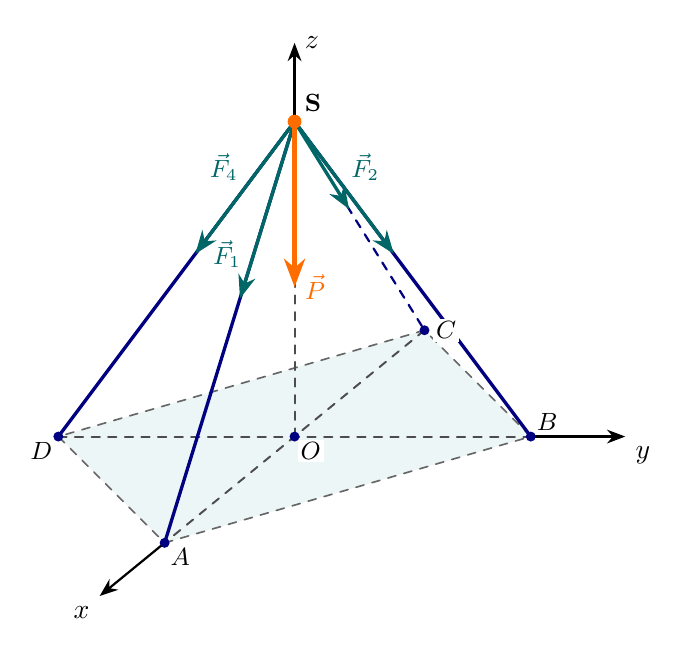
\begin{tikzpicture}[scale=1.0, >=Stealth, line join=round, line cap=round,
    x={(-0.55cm,-0.45cm)}, y={(1cm,0cm)}, z={(0cm,1cm)}]
    \coordinate (O) at (0,0,0);
    \coordinate (S) at (0,0,4);
    \coordinate (A) at (3,0,0);
    \coordinate (B) at (0,3,0);
    \coordinate (C) at (-3,0,0);
    \coordinate (D) at (0,-3,0);

    \fill[teal!10, opacity=0.7] (A) -- (B) -- (C) -- (D) -- cycle;
    \draw[dashed, black!60, line width=0.6pt] (A) -- (B) -- (C) -- (D) -- cycle;

    \draw[dashed, black!70, line width=0.7pt] (C) -- (A);
    \draw[dashed, black!70, line width=0.7pt] (D) -- (B);
    \draw[dashed, black!70, line width=0.7pt] (O) -- (S);

    \draw[->, thick, black] (A) -- (4.5,0,0) node[below left] {$x$};
    \draw[->, thick, black] (B) -- (0,4.2,0) node[below right] {$y$};
    \draw[->, thick, black] (S) -- (0,0,5.0) node[right] {$z$};

    \draw[dashed, thick, blue!50!black] (S) -- (C);
    \draw[very thick, blue!50!black] (S) -- (A);
    \draw[very thick, blue!50!black] (S) -- (B);
    \draw[very thick, blue!50!black] (S) -- (D);

    \draw[->, very thick, teal!80!black] (S) -- ($(S)!0.42!(A)$) node[pos=0.75, left=3pt, fill=white, inner sep=1pt] {\small $\vec{F}_1$};
    \draw[->, very thick, teal!80!black] (S) -- ($(S)!0.42!(B)$) node[midway, above right=1pt, fill=white, inner sep=1pt] {\small $\vec{F}_2$};
    \draw[->, very thick, teal!80!black] (S) -- ($(S)!0.42!(C)$);
    \draw[->, very thick, teal!80!black] (S) -- ($(S)!0.42!(D)$) node[midway, above left=1pt, fill=white, inner sep=1pt] {\small $\vec{F}_4$};

    \draw[->, ultra thick, orange!85!red] (S) -- (0,0,1.9) node[right=2pt, fill=white, inner sep=1pt] {\small $\vec{P}$};

    \foreach \p in {A,B,C,D,O} \fill[blue!50!black] (\p) circle (1.8pt);
    \fill[orange!85!red] (S) circle (2.5pt);

    \node[below right=1pt, fill=white, inner sep=1pt] at (O) {\small $O$};
    \node[above right=2pt, fill=white, inner sep=1.5pt] at (S) {\small $\mathbf{S}$};
    \node[below right=1pt, fill=white, inner sep=1pt] at (A) {\small $A$};
    \node[above right=1pt, fill=white, inner sep=1pt] at (B) {\small $B$};
    \node[right=3pt, fill=white, inner sep=1pt] at (C) {\small $C$};
    \node[below left=1pt, fill=white, inner sep=1pt] at (D) {\small $D$};
\end{tikzpicture}%
}
\end{minipage}
\vspace{0.2cm}

\item \begin{minipage}[t]{0.55\linewidth}
Ông An có một khu đất hình elip với độ dài trục lớn bằng $10\text{ m}$ và độ dài trục bé bằng $8\text{ m}$. Ông An muốn chia khu đất thành hai phần (như hình vẽ): phần hình chữ nhật nội tiếp elip (có các cạnh song song với các trục của elip, phần tô đậm) dùng để xây bể cá cảnh, và phần diện tích còn lại xung quanh (phần gạch chéo) dùng để trồng hoa. Biết chi phí xây bể cá cảnh là $800.000\text{ đồng/m}^2$ và chi phí trồng hoa là $900.000\text{ đồng/m}^2$. Hỏi ông An có thể thiết kế xây dựng như trên với tổng chi phí thấp nhất là bao nhiêu triệu đồng (làm tròn kết quả đến hàng phần trăm)?
\end{minipage}\hfill
\begin{minipage}[t]{0.42\linewidth}
\vspace{-0.4\baselineskip}
\centering
\resizebox{0.95\linewidth}{!}{%
\begin{tikzpicture}[>=Stealth, line join=round, line cap=round, scale=0.52]
    % Elip voi ban truc a=5, b=4: to mau cam nhat + gach cheo de vua co mau dep vua in trang den ro net
    \fill[orange!15] (0,0) ellipse (5cm and 4cm);
    \fill[pattern=north east lines, pattern color=orange!80!black] (0,0) ellipse (5cm and 4cm);
    \draw[very thick, blue!55!black] (0,0) ellipse (5cm and 4cm);

    % Hinh chu nhat noi tiep: to mau teal dam vua phai
    \fill[white] (-3.535,-2.828) rectangle (3.535,2.828);
    \fill[teal!22] (-3.535,-2.828) rectangle (3.535,2.828);
    \draw[very thick, teal!80!black] (-3.535,-2.828) rectangle (3.535,2.828);

    % Truc toa do Oxy chuan SGK
    \draw[->, thick, black] (-6.0,0) -- (6.2,0) node[below] {\large $x$};
    \draw[->, thick, black] (0,-4.9) -- (0,5.2) node[right] {\large $y$};
    \node[below left=1pt] at (0,0) {$O$};

    % Nhan truc va chu thich truc tiep
    \node[below right=1pt, fill=white, inner sep=1pt] at (5,0) {$5$};
    \node[below left=1pt, fill=white, inner sep=1pt] at (-5,0) {$-5$};
    \node[above right=1pt, fill=white, inner sep=1pt] at (0,4) {$4$};
    \node[below right=1pt, fill=white, inner sep=1pt] at (0,-4) {$-4$};

    \node[fill=white, inner sep=2pt, rounded corners=1pt, text=teal!80!black] at (0,1.0) {\textbf{Bể cá cảnh}};
    \draw[<-, thick, black] (2.2,3.25) -- (3.8,4.3) node[right, fill=white, inner sep=1pt] {\small Trồng hoa};
\end{tikzpicture}%
}
\end{minipage}
\vspace{0.2cm}

\item \begin{minipage}[t]{0.55\linewidth}
Trong không gian $Oxyz$ (đơn vị trên mỗi trục tọa độ là mét), một thiết bị phát tia laser được đặt cố định tại điểm $A(6; 3; 4)$. Thiết bị này chiếu một tia sáng về phía bức tường phẳng trùng với mặt phẳng tọa độ $(Oyz)$. Biết rằng tia sáng phát ra có thể xoay theo mọi hướng nhưng luôn tạo với trục $Ox$ một góc $45^\circ$. Gọi $M$ là vị trí vệt sáng laser chiếu lên bức tường $(Oyz)$. Khoảng cách lớn nhất từ vệt sáng $M$ đến gốc tọa độ $O$ bằng bao nhiêu mét?
\end{minipage}\hfill
\begin{minipage}[t]{0.42\linewidth}
\vspace{-0.4\baselineskip}
\centering
\resizebox{0.92\linewidth}{!}{%
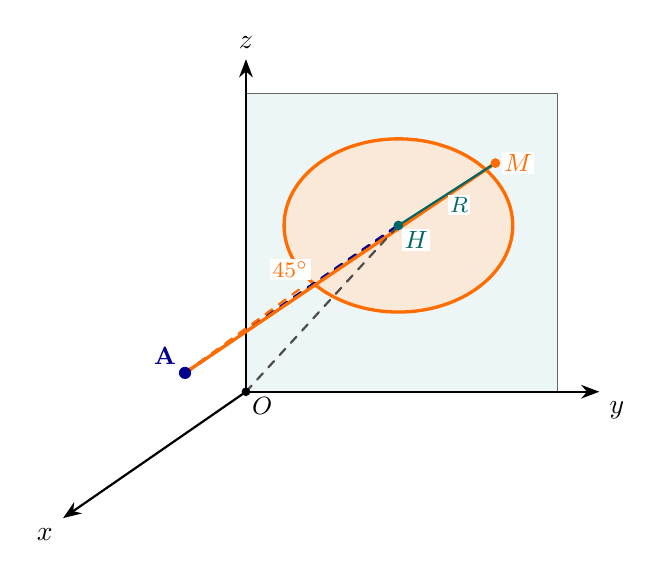
\begin{tikzpicture}[>=Stealth, line join=round, line cap=round,
    x={(-0.55cm,-0.38cm)}, y={(1cm,0cm)}, z={(0cm,1cm)}, scale=0.88]
    \coordinate (O) at (0,0,0);
    \coordinate (H) at (0,2.2,2.4);
    \coordinate (A) at (5.6,2.2,2.4);
    \coordinate (M1) at (0,3.6,3.3);
    \coordinate (M2) at (0,0.8,1.5);

    % Buc tuong phang (Oyz) ben phai truc Oz
    \fill[teal!10, opacity=0.7] (0,0,0) -- (0,4.5,0) -- (0,4.5,4.3) -- (0,0,4.3) -- cycle;
    \draw[black!60, thin] (0,0,0) -- (0,4.5,0) -- (0,4.5,4.3) -- (0,0,4.3) -- cycle;

    % Duong tron quy tich vet sang M tren tuong (Oyz)
    \fill[orange!20, opacity=0.7] (H) circle[x radius=1.65cm, y radius=1.25cm];
    \draw[very thick, orange!85!red] (H) circle[x radius=1.65cm, y radius=1.25cm];

    % Truc Oxyz chuan SGK
    \draw[->, thick, black] (O) -- (4.8,0,0) node[below left] {$x$};
    \draw[->, thick, black] (O) -- (0,5.1,0) node[below right] {$y$};
    \draw[->, thick, black] (O) -- (0,0,4.8) node[above] {$z$};

    % Truc chuan AH // Ox va tia laser AM
    \draw[dashed, very thick, blue!55!black] (A) -- (H);
    \draw[very thick, orange!85!red] (A) -- (M1) node[pos=0.42, above left=1pt, fill=white, inner sep=1pt] {\footnotesize $45^\circ$};
    \draw[dashed, thick, orange!85!red] (A) -- (M2);
    \draw[thick, teal!80!black] (H) -- (M1) node[midway, below right=0pt, fill=white, inner sep=0.8pt] {\footnotesize $R$};
    \draw[dashed, thick, black!70] (O) -- (H);

    % Chi ghi ten diem O, H, M, A ngan gon
    \fill[black] (O) circle (1.8pt) node[below right=1pt, fill=white, inner sep=1pt] {\small $O$};
    \fill[teal!80!black] (H) circle (2.0pt) node[below right=1pt, fill=white, inner sep=1pt] {\small $H$};
    \fill[orange!85!red] (M1) circle (2.0pt) node[right=2pt, fill=white, inner sep=1pt] {\small $M$};
    \fill[blue!55!black] (A) circle (2.5pt) node[above left=2pt, fill=white, inner sep=1pt] {\small $\mathbf{A}$};
\end{tikzpicture}%
}
\end{minipage}
\vspace{0.2cm}

\item Có hai hộp đựng bi: Hộp I chứa $4$ viên bi đỏ và $6$ viên bi xanh; Hộp II chứa $7$ viên bi đỏ và $3$ viên bi xanh. Bạn Bình tung một đồng xu cân đối và đồng chất: nếu đồng xu xuất hiện mặt sấp thì Bình lấy ngẫu nhiên đồng thời $2$ viên bi từ Hộp I; nếu đồng xu xuất hiện mặt ngửa thì Bình lấy ngẫu nhiên đồng thời $2$ viên bi từ Hộp II. Biết rằng $2$ viên bi mà Bình lấy ra đều có màu đỏ, xác suất để $2$ viên bi đó được lấy từ Hộp II là phân số tối giản $\dfrac{a}{b}$ với $a, b \in \mathbb{N}^*$. Tính giá trị của tổng $T = a + b$.

\item \begin{minipage}[t]{0.55\linewidth}
Một họa sĩ thiết kế logo hình con cá cho một doanh nghiệp thủy sản trên hệ trục tọa độ $Oxy$ (đơn vị trên mỗi trục là centimét). Đường viền của logo được giới hạn bởi hai parabol đối xứng nhau qua trục hoành là $y = 4 - \dfrac{1}{4}x^2$ và $y = \dfrac{1}{4}x^2 - 4$, tính từ đầu cá tại $x = -4$ qua nút thắt giao điểm tại $x = 4$ đến mép thẳng đứng của đuôi cá tại đường thẳng $x = 6$ (gồm phần thân cá tô đậm và phần đuôi cá gạch chéo như hình vẽ). Tổng diện tích của toàn bộ logo hình con cá bằng bao nhiêu $\text{cm}^2$?
\end{minipage}\hfill
\begin{minipage}[t]{0.42\linewidth}
\vspace{-0.4\baselineskip}
\centering
\resizebox{\linewidth}{!}{%
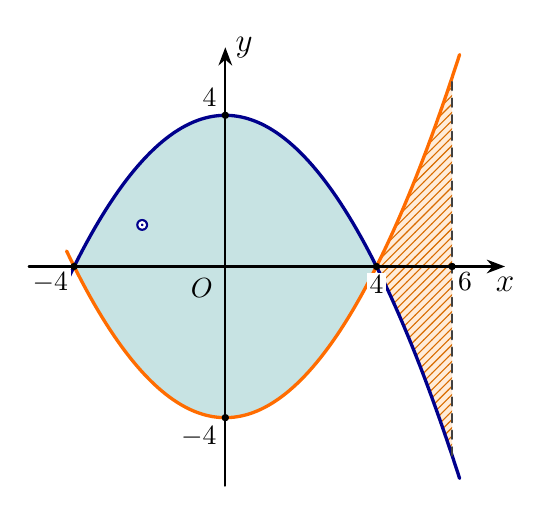
\begin{tikzpicture}[>=Stealth, line join=round, line cap=round, scale=0.48]
    % To mau teal + dam phan than ca [-4, 4]
    \fill[teal!22] plot[domain=-4:4, samples=80] (\x, {4 - 0.25*\x*\x})
        -- plot[domain=4:-4, samples=80] (\x, {0.25*\x*\x - 4}) -- cycle;

    % To mau cam nhat + gach cheo phan duoi ca [4, 6]
    \fill[orange!15]
        plot[domain=4:6, samples=40] (\x, {0.25*\x*\x - 4})
        -- (6,-5)
        -- plot[domain=6:4, samples=40] (\x, {4 - 0.25*\x*\x}) -- cycle;
    \fill[pattern=north east lines, pattern color=orange!85!black]
        plot[domain=4:6, samples=40] (\x, {0.25*\x*\x - 4})
        -- (6,-5)
        -- plot[domain=6:4, samples=40] (\x, {4 - 0.25*\x*\x}) -- cycle;

    % Hai duong parabol va duong thang x = 6 (khong ghi phuong trinh len hinh de hoc sinh tu nhan biet)
    \draw[very thick, blue!55!black, domain=-4.2:6.2, samples=100] plot (\x, {4 - 0.25*\x*\x});
    \draw[very thick, orange!85!red, domain=-4.2:6.2, samples=100] plot (\x, {0.25*\x*\x - 4});
    \draw[thick, dashed, black!75] (6,-5) -- (6,5);

    % Mat ca trang tri
    \fill[blue!55!black] (-2.2,1.1) circle (4.5pt);
    \draw[thick, white] (-2.2,1.1) circle (2.0pt);

    % Truc toa do Oxy chuan SGK
    \draw[->, thick, black] (-5.2,0) -- (7.4,0) node[below] {\large $x$};
    \draw[->, thick, black] (0,-5.8) -- (0,5.8) node[right] {\large $y$};
    \node[below left=1pt] at (0,0) {$O$};

    % Chi hien thi cac moc toa do tren truc (hoc sinh tu nhan dien duong cong)
    \fill[black] (-4,0) circle (2.8pt) node[below left=1pt, fill=white, inner sep=1pt] {$-4$};
    \fill[black] (4,0) circle (2.8pt) node[below=2pt, fill=white, inner sep=1pt] {$4$};
    \fill[black] (6,0) circle (2.8pt) node[below right=1pt, fill=white, inner sep=1pt] {$6$};
    \fill[black] (0,4) circle (2.8pt) node[above left=2pt, fill=white, inner sep=1pt] {$4$};
    \fill[black] (0,-4) circle (2.8pt) node[below left=2pt, fill=white, inner sep=1pt] {$-4$};
\end{tikzpicture}%
}
\end{minipage}

\end{enumerate}

\newpage
% ==========================================
% BẢNG ĐÁP ÁN TỔNG HỢP
% ==========================================
\section*{BẢNG ĐÁP ÁN TỔNG HỢP}

\subsection*{1. PHẦN I}
\begin{center}
\begin{tabular}{|c|c||c|c||c|c||c|c|}
\hline
\textbf{Câu} & \textbf{Đáp án} & \textbf{Câu} & \textbf{Đáp án} & \textbf{Câu} & \textbf{Đáp án} & \textbf{Câu} & \textbf{Đáp án} \\ \hline
1 & A & 4 & B & 7 & B & 10 & C \\ \hline
2 & C & 5 & A & 8 & D & 11 & B \\ \hline
3 & D & 6 & C & 9 & A & 12 & D \\ \hline
\end{tabular}
\end{center}

\subsection*{2. PHẦN II}
\begin{center}
\begin{tabular}{|c|c|c|c|c|}
\hline
\textbf{Câu} & \textbf{Ý a)} & \textbf{Ý b)} & \textbf{Ý c)} & \textbf{Ý d)} \\ \hline
\textbf{1} & Đúng & Đúng & Sai & Đúng \\ \hline
\textbf{2} & Đúng & Sai & Đúng & Đúng \\ \hline
\textbf{3} & Đúng & Đúng & Sai & Đúng \\ \hline
\textbf{4} & Đúng & Sai & Đúng & Đúng \\ \hline
\end{tabular}
\end{center}

\subsection*{3. PHẦN III}
\begin{center}
\begin{tabular}{|c|c||c|c||c|c|}
\hline
\textbf{Câu} & \textbf{Kết quả điền} & \textbf{Câu} & \textbf{Kết quả điền} & \textbf{Câu} & \textbf{Kết quả điền} \\ \hline
\textbf{1} & 11,18 & \textbf{3} & 52,55 & \textbf{5} & 16 \\ \hline
\textbf{2} & 25 & \textbf{4} & 11 & \textbf{6} & 52 \\ \hline
\end{tabular}
\end{center}

\newpage
% ==========================================
% HƯỚNG DẪN GIẢI CHI TIẾT
% ==========================================
\section*{HƯỚNG DẪN GIẢI CHI TIẾT}

\subsection*{PHẦN I}
\begin{enumerate}[label=\textbf{Câu \arabic*:}, leftmargin=*]

\item \textbf{Đáp án A.}
Tập xác định: $D = \mathbb{R} \setminus \{m\}$.\\
Ta viết lại hàm số dưới dạng:
$$y = \dfrac{(x - m)^2 + m - 2}{x - m} = x - m + \dfrac{m - 2}{x - m}.$$
Đạo hàm:
$$y' = 1 - \dfrac{m - 2}{(x - m)^2} = \dfrac{(x - m)^2 - (m - 2)}{(x - m)^2}.$$
Đồ thị hàm số có hai điểm cực trị khi và chỉ khi phương trình $y' = 0$ có hai nghiệm phân biệt khác $m$, tức là $m - 2 > 0 \iff m > 2$.\\
Khi đó hoành độ hai điểm cực trị $A, B$ là $x_1 = m - \sqrt{m - 2}$ và $x_2 = m + \sqrt{m - 2}$, suy ra $x_2 - x_1 = 2\sqrt{m - 2}$.\\
Đường thẳng đi qua hai điểm cực trị có phương trình $y = \dfrac{(x^2 - 2mx + m^2 + m - 2)'}{(x - m)'} = 2x - 2m$, do đó $y_2 - y_1 = 2(x_2 - x_1)$.\\
Bình phương độ dài đoạn thẳng $AB$ là:
$$AB^2 = (x_2 - x_1)^2 + (y_2 - y_1)^2 = 5(x_2 - x_1)^2 = 5 \cdot 4(m - 2) = 20(m - 2).$$
Theo giả thiết $AB \le 2\sqrt{15} \iff 20(m - 2) \le 60 \iff m - 2 \le 3 \iff m \le 5$.\\
Kết hợp điều kiện $m > 2$ và $m \in \mathbb{Z}$, ta được $m \in \{3; 4; 5\}$. Vậy có $3$ giá trị nguyên của $m$.

\item \textbf{Đáp án C.}
Điều kiện xác định: $\begin{cases} x - 1 > 0 \\ 9 - x > 0 \end{cases} \iff 1 < x < 9$.\\
Bất phương trình tương đương với:
$$\log_2\left[(x - 1)(9 - x)\right] \ge 3 \iff -x^2 + 10x - 9 \ge 2^3 = 8 \iff x^2 - 10x + 17 \le 0.$$
Giải bất phương trình bậc hai ta được $5 - 2\sqrt{2} \le x \le 5 + 2\sqrt{2}$ (xấp xỉ $2{,}17 \le x \le 7{,}83$), thỏa mãn điều kiện $1 < x < 9$.\\
Vì $x \in \mathbb{Z}$ nên $x \in \{3; 4; 5; 6; 7\}$. Vậy bất phương trình có $5$ nghiệm nguyên.

\item \textbf{Đáp án D.}
Nhận thấy vế trái của đẳng thức là đạo hàm của tích $[x f(x)]' = f(x) + x f'(x)$.\\
Do đó:
$$[x f(x)]' = 4x^3 - 6x^2 + 2x + 1 \implies x f(x) = \int (4x^3 - 6x^2 + 2x + 1)\,\mathrm{d}x = x^4 - 2x^3 + x^2 + x + C.$$
Thay $x = 0$ vào hai vế (do $f(x)$ liên tục trên $\mathbb{R}$) ta suy ra $C = 0$, dẫn đến:
$$f(x) = x^3 - 2x^2 + x + 1, \quad \forall x \in \mathbb{R}.$$
Vậy tích phân cần tính là:
$$I = \int_0^2 (x^3 - 2x^2 + x + 1)\,\mathrm{d}x = \left[ \dfrac{x^4}{4} - \dfrac{2x^3}{3} + \dfrac{x^2}{2} + x \right]_0^2 = 4 - \dfrac{16}{3} + 2 + 2 = \dfrac{8}{3}.$$

\item \textbf{Đáp án B.}
Vì $N \in \Delta$ nên gọi tọa độ điểm $N(4 + 2t; -2 - t; 4 + t)$.\\
Do $N$ là trung điểm của đoạn thẳng $AM$ với $A(2; -1; 3)$ nên tọa độ điểm $M$ là:
$$\begin{cases} x_M = 2x_N - x_A = 6 + 4t \\ y_M = 2y_N - y_A = -3 - 2t \\ z_M = 2z_N - z_A = 5 + 2t \end{cases} \implies M(6 + 4t; -3 - 2t; 5 + 2t).$$
Vì $M \in (P): x - y - 2z + 4 = 0$ nên ta có:
$$(6 + 4t) - (-3 - 2t) - 2(5 + 2t) + 4 = 0 \iff 2t + 3 = 0 \iff t = -\dfrac{3}{2}.$$
Suy ra $N\left(1; -\dfrac{1}{2}; \dfrac{5}{2}\right)$, do đó $\overrightarrow{AN} = \left(-1; \dfrac{1}{2}; -\dfrac{1}{2}\right) = -\dfrac{1}{2}(2; -1; 1)$.\\
Vậy đường thẳng $d$ nhận $\vec{u}_2 = (2; -1; 1)$ làm một vectơ chỉ phương.

\item \textbf{Đáp án A.}
Gọi $B$ là biến cố ``An đi học bằng xe buýt'' $\implies P(B) = 0{,}40$ và $P(\overline{B}) = 0{,}60$.\\
Gọi $M$ là biến cố ``An bị muộn học''. Theo giả thiết: $P(M \mid B) = 0{,}06$ và $P(M \mid \overline{B}) = 0{,}02$.\\
Theo công thức xác suất toàn phần, xác suất An bị muộn học là:
$$P(M) = P(B)P(M \mid B) + P(\overline{B})P(M \mid \overline{B}) = 0{,}40 \times 0{,}06 + 0{,}60 \times 0{,}02 = 0{,}024 + 0{,}012 = 0{,}036.$$
Theo công thức Bayes, xác suất An đã đi bằng xe buýt khi biết bị muộn học là:
$$P(B \mid M) = \dfrac{P(B)P(M \mid B)}{P(M)} = \dfrac{0{,}024}{0{,}036} = \dfrac{2}{3}.$$

\item \textbf{Đáp án C.}
Cỡ mẫu $N = 6 + 12 + 10 + 8 + 4 = 40$. Giá trị đại diện của các nhóm lần lượt là $5; 7; 9; 11; 13$.\\
Số trung bình cộng của mẫu số liệu ghép nhóm là:
$$\bar{x} = \dfrac{6 \cdot 5 + 12 \cdot 7 + 10 \cdot 9 + 8 \cdot 11 + 4 \cdot 13}{40} = \dfrac{344}{40} = 8{,}6\text{ (kg)}.$$
Phương sai của mẫu số liệu ghép nhóm là:
$$s^2 = \dfrac{6(5 - 8{,}6)^2 + 12(7 - 8{,}6)^2 + 10(9 - 8{,}6)^2 + 8(11 - 8{,}6)^2 + 4(13 - 8{,}6)^2}{40} = 5{,}84.$$

\item \textbf{Đáp án B.}
Hàm số $f(x) = (x^2 - 5x + 7)e^x$ liên tục và xác định trên đoạn $[0; 3]$.\\
Đạo hàm:
$$f'(x) = (2x - 5)e^x + (x^2 - 5x + 7)e^x = (x^2 - 3x + 2)e^x.$$
Trên đoạn $[0; 3]$, $f'(x) = 0 \iff x = 1$ hoặc $x = 2$.\\
Tính giá trị tại các điểm đầu mút và điểm tới hạn:
$$f(0) = 7; \quad f(1) = 3e \approx 8{,}15; \quad f(2) = e^2 \approx 7{,}39; \quad f(3) = e^3 \approx 20{,}09.$$
Vậy $\max\limits_{[0; 3]} f(x) = f(3) = e^3$.

\item \textbf{Đáp án D.}
Phương trình hoành độ giao điểm của $(P)$ và $d$:
$$x^2 - 4x + 3 = x - 1 \iff x^2 - 5x + 4 = 0 \iff \begin{bmatrix} x = 1 \\ x = 4 \end{bmatrix}.$$
Diện tích hình phẳng giới hạn bởi hai đồ thị là:
$$S = \int_1^4 \left|x^2 - 5x + 4\right|\,\mathrm{d}x = \int_1^4 (-x^2 + 5x - 4)\,\mathrm{d}x = \left[ -\dfrac{x^3}{3} + \dfrac{5x^2}{2} - 4x \right]_1^4 = \dfrac{9}{2}.$$

\item \textbf{Đáp án A.}
Gọi $I$ là điểm thỏa mãn $2\overrightarrow{IA} + \overrightarrow{IB} = \vec{0}$. Tọa độ điểm $I$ là:
$$I = \dfrac{2A + B}{3} = \left(\dfrac{2\cdot 1 + 4}{3}; \dfrac{2\cdot 2 - 1}{3}; \dfrac{2\cdot 1 + 4}{3}\right) = (2; 1; 2).$$
Khi đó với mọi điểm $M \in (P)$, ta có:
$$T = 2\left(\overrightarrow{MI} + \overrightarrow{IA}\right)^2 + \left(\overrightarrow{MI} + \overrightarrow{IB}\right)^2 = 3MI^2 + 2IA^2 + IB^2.$$
Do $I, A, B$ cố định nên $T$ đạt giá trị nhỏ nhất khi và chỉ khi $MI$ nhỏ nhất, tức $M$ là hình chiếu vuông góc của $I(2; 1; 2)$ lên mặt phẳng $(P): 2x - y + 2z - 16 = 0$.\\
Đường thẳng qua $I$ vuông góc với $(P)$ có phương trình tham số: $x = 2 + 2t, y = 1 - t, z = 2 + 2t$.\\
Thay vào phương trình mặt phẳng $(P)$:
$$2(2 + 2t) - (1 - t) + 2(2 + 2t) - 16 = 0 \iff 9t - 9 = 0 \iff t = 1.$$
Suy ra tọa độ $M(4; 0; 4)$, do đó $a + b + c = 4 + 0 + 4 = 8$.

\item \textbf{Đáp án C.}
Theo tính chất của cấp số cộng, ta có $u_3 + u_4 = u_2 + u_5 = 24$.\\
Kết hợp với $u_3 \cdot u_4 = 135$ và $d > 0$ (suy ra $u_3 < u_4$), ta tìm được $u_3 = 9$ và $u_4 = 15$.\\
Từ đó công sai $d = u_4 - u_3 = 6$ và số hạng đầu $u_1 = u_3 - 2d = 9 - 12 = -3$.\\
Tổng $10$ số hạng đầu tiên là:
$$S_{10} = \dfrac{10\left(2u_1 + 9d\right)}{2} = 5\left[2(-3) + 9\cdot 6\right] = 5 \cdot 48 = 240.$$

\item \textbf{Đáp án B.}
Tọa độ trung điểm $P$ của $AB$ và trung điểm $Q$ của $CD$ lần lượt là:
$$P\left(\dfrac{2+4}{2}; \dfrac{-1+3}{2}; \dfrac{1-1}{2}\right) = (3; 1; 0), \quad Q\left(\dfrac{1+5}{2}; \dfrac{2+4}{2}; \dfrac{4+6}{2}\right) = (3; 3; 5).$$
Độ dài đoạn thẳng $PQ$ là:
$$PQ = \sqrt{(3 - 3)^2 + (3 - 1)^2 + (5 - 0)^2} = \sqrt{0 + 4 + 25} = \sqrt{29}.$$

\item \textbf{Đáp án D.}
Tổng số học sinh của đội là $6 + 5 + 4 = 15$ học sinh. Số phần tử của không gian mẫu là $n(\Omega) = C_{15}^4 = 1365$.\\
Để $4$ học sinh được chọn có mặt đủ cả $3$ khối và số học sinh khối 12 nhiều hơn số học sinh khối 10, chỉ có duy nhất trường hợp chọn được: $2$ học sinh khối 12, $1$ học sinh khối 11 và $1$ học sinh khối 10.\\
Số cách chọn thuận lợi là: $n(A) = C_6^2 \cdot C_5^1 \cdot C_4^1 = 15 \cdot 5 \cdot 4 = 300$.\\
Xác suất cần tìm là $P(A) = \dfrac{300}{1365} = \dfrac{20}{91}$.

\end{enumerate}

\subsection*{PHẦN II}
\begin{enumerate}[label=\textbf{Câu \arabic*:}, leftmargin=*]

\item \textbf{Đáp án: a) Đúng | b) Đúng | c) Sai | d) Đúng.}
\begin{itemize}[leftmargin=*]
    \item \textbf{Ý a) Đúng:} Tổng doanh thu là $R(x) = x \cdot p(x) = x(-x^2 + 9x + 120) = -x^3 + 9x^2 + 120x$ (triệu đồng).
    \item \textbf{Ý b) Đúng:} Hàm lợi nhuận ròng là $L(x) = R(x) - C(x) = (-x^3 + 9x^2 + 120x) - (72x + 100) = -x^3 + 9x^2 + 48x - 100$. Đạo hàm $L'(x) = -3x^2 + 18x + 48$.
    \item \textbf{Ý c) Sai:} Cho $L'(x) = 0 \iff -3(x - 8)(x + 2) = 0 \implies x = 8$ (do $x > 0$). Khi không bị giới hạn công suất, lợi nhuận đạt cực đại tại $x = 8$ ngàn thiết bị với $L(8) = 348$ triệu đồng (chứ không phải tại $x = 6$).
    \item \textbf{Ý d) Đúng:} Trên miền công suất giới hạn $x \in (0; 6]$, ta có $L'(x) = -3(x - 8)(x + 2) > 0$ với mọi $x \in (0; 6]$, nên hàm số $L(x)$ đồng biến nghiêm ngặt trên $(0; 6]$. Do đó lợi nhuận lớn nhất đạt tại biên $x = 6$ ngàn thiết bị với $L(6) = -6^3 + 9\cdot 6^2 + 48\cdot 6 - 100 = 296$ triệu đồng.
\end{itemize}

\item \textbf{Đáp án: a) Đúng | b) Sai | c) Đúng | d) Đúng.}
\begin{itemize}[leftmargin=*]
    \item \textbf{Ý a) Đúng:} Trong $600$ học sinh có $400$ học sinh thích học Toán nên $P(T) = \dfrac{400}{600} = \dfrac{2}{3}$ và $P(\overline{T}) = \dfrac{200}{600} = \dfrac{1}{3}$.
    \item \textbf{Ý b) Sai:} Theo đề bài, tỉ lệ giỏi Toán trong nhóm không thích học Toán là $15\%$ nên $P(G \mid \overline{T}) = 0{,}15 \ne 0{,}25$.
    \item \textbf{Ý c) Đúng:} Áp dụng công thức xác suất toàn phần:
    $$P(G) = P(T)P(G \mid T) + P(\overline{T})P(G \mid \overline{T}) = \dfrac{2}{3} \cdot 0{,}75 + \dfrac{1}{3} \cdot 0{,}15 = 0{,}50 + 0{,}05 = 0{,}55.$$
    \item \textbf{Ý d) Đúng:} Áp dụng công thức Bayes:
    $$P(T \mid G) = \dfrac{P(T)P(G \mid T)}{P(G)} = \dfrac{0{,}50}{0{,}55} = \dfrac{10}{11} \approx 90{,}91\%.$$
\end{itemize}

\item \textbf{Đáp án: a) Đúng | b) Đúng | c) Sai | d) Đúng.}
\begin{itemize}[leftmargin=*]
    \item \textbf{Ý a) Đúng:} Từ $L_A = 10\log_{10}\!\left(\dfrac{I_A}{10^{-12}}\right) = 80 \implies \log_{10}\!\left(\dfrac{I_A}{10^{-12}}\right) = 8 \implies I_A = 10^{-12} \cdot 10^8 = 10^{-4}\text{ W/m}^2$.
    \item \textbf{Ý b) Đúng:} Từ $L_B = 90\text{ dB} \implies I_B = 10^{-12} \cdot 10^9 = 10^{-3}\text{ W/m}^2 = 10 I_A$.
    \item \textbf{Ý c) Sai:} Khi bật cả hai loa, cường độ âm cộng tuyến tính ($I = I_A + I_B$), còn mức cường độ âm tính theo hàm logarit nên không thể lấy $L_A + L_B = 170\text{ dB}$.
    \item \textbf{Ý d) Đúng:} Cường độ âm tổng hợp là $I = I_A + I_B = 10^{-4} + 10^{-3} = 1{,}1 \cdot 10^{-3}\text{ W/m}^2$. Mức cường độ âm tổng hợp là:
    $$L = 10\log_{10}\!\left(\dfrac{1{,}1 \cdot 10^{-3}}{10^{-12}}\right) = 10\log_{10}(1{,}1 \cdot 10^9) = 90 + 10\log_{10}(1{,}1) \approx 90{,}41\text{ dB}.$$
\end{itemize}

\item \textbf{Đáp án: a) Đúng | b) Sai | c) Đúng | d) Đúng.}
\begin{itemize}[leftmargin=*]
    \item \textbf{Ý a) Đúng:} $\overrightarrow{AB} = (3; 10; 8) \implies AB = \sqrt{3^2 + 10^2 + 8^2} = \sqrt{173}\text{ km}$.
    \item \textbf{Ý b) Sai:} Với $M(x; y; 5)$ và $A(1; 1; 5)$, điều kiện $MA = 5\text{ km}$ tương đương $MA^2 = 25 \iff (x - 1)^2 + (y - 1)^2 + (5 - 5)^2 = 25$ (chứ không phải bằng $5$).
    \item \textbf{Ý c) Đúng:} Từ $MA = 5, MB = 10, MC = 13$ với $z_M = 5$, ta có hệ phương trình:
    $$\begin{cases} (x - 1)^2 + (y - 1)^2 = 25 \quad (1) \\ (x - 4)^2 + (y - 11)^2 + 8^2 = 100 \iff (x - 4)^2 + (y - 11)^2 = 36 \quad (2) \\ (x - 16)^2 + (y - 5)^2 + 5^2 = 169 \iff (x - 16)^2 + (y - 5)^2 = 144 \quad (3) \end{cases}$$
    Lấy $(1)$ trừ $(2)$ và $(1)$ trừ $(3)$ thu được hệ bậc nhất:
    $$\begin{cases} 3x + 10y = 62 \\ 15x + 4y = 140 \end{cases} \iff \begin{cases} x = 4 \\ y = 5 \end{cases} \implies M(4; 5; 5).$$
    \item \textbf{Ý d) Đúng:} Khoảng cách từ $M(4; 5; 5)$ đến gốc $O(0; 0; 0)$ là $OM = \sqrt{4^2 + 5^2 + 5^2} = \sqrt{66} \approx 8{,}12\text{ km}$.
\end{itemize}

\end{enumerate}

\subsection*{PHẦN III}
\begin{enumerate}[label=\textbf{Câu \arabic*:}, leftmargin=*]

\item \textbf{Đáp số: 11,18}
Gọi $H$ là hình chiếu vuông góc của cọc $K$ lên bờ $AC$, ta có $AH = 1\text{ m}$ và $KH = 8\text{ m}$.\\
Đặt $HQ = x\text{ (m)}$ với $x > 0$, suy ra $AQ = x + 1\text{ (m)}$.\\
Do $KH \parallel AP$ nên theo định lý Thales:
$$\dfrac{AP}{KH} = \dfrac{AQ}{HQ} \implies AP = \dfrac{8(x + 1)}{x}\text{ (m)}.$$
Bình phương chiều dài cây sào $PQ$ là:
$$f(x) = PQ^2 = AQ^2 + AP^2 = (x + 1)^2 + \dfrac{64(x + 1)^2}{x^2} = (x + 1)^2\left(1 + \dfrac{64}{x^2}\right).$$
Lấy đạo hàm:
$$f'(x) = 2(x + 1)\left(1 + \dfrac{64}{x^2}\right) + (x + 1)^2\left(-\dfrac{128}{x^3}\right) = \dfrac{2(x + 1)(x^3 - 64)}{x^3}.$$
Cho $f'(x) = 0$ với $x > 0 \iff x^3 = 64 \iff x = 4\text{ m}$.\\
Khi đó chiều dài ngắn nhất của cây sào là:
$$PQ_{\min} = \sqrt{f(4)} = 5\sqrt{1 + \dfrac{64}{16}} = 5\sqrt{5} \approx 11{,}18\text{ (m)}.$$

\item \textbf{Đáp số: 25}
Ta có tọa độ các vectơ chân giá đỡ xuất phát từ đỉnh $S(0; 0; 40)$:
$$\overrightarrow{SA} = (30; 0; -40), \quad \overrightarrow{SB} = (0; 30; -40), \quad \overrightarrow{SC} = (-30; 0; -40), \quad \overrightarrow{SD} = (0; -30; -40).$$
Độ dài mỗi thanh giá đỡ là:
$$SA = SB = SC = SD = \sqrt{30^2 + 0^2 + (-40)^2} = 50\text{ (cm)}.$$
Vì bốn lực $\vec{F}_1, \vec{F}_2, \vec{F}_3, \vec{F}_4$ cùng độ lớn $F$ và hướng dọc theo các vectơ $\overrightarrow{SA}, \overrightarrow{SB}, \overrightarrow{SC}, \overrightarrow{SD}$ nên:
$$\vec{F}_1 = \dfrac{F}{50}\overrightarrow{SA}, \quad \vec{F}_2 = \dfrac{F}{50}\overrightarrow{SB}, \quad \vec{F}_3 = \dfrac{F}{50}\overrightarrow{SC}, \quad \vec{F}_4 = \dfrac{F}{50}\overrightarrow{SD}.$$
Cộng bốn vectơ lực lại ta được:
$$\vec{P} = \vec{F}_1 + \vec{F}_2 + \vec{F}_3 + \vec{F}_4 = \dfrac{F}{50}\left(\overrightarrow{SA} + \overrightarrow{SB} + \overrightarrow{SC} + \overrightarrow{SD}\right) = \dfrac{F}{50}(0; 0; -160) = \left(0; 0; -\dfrac{16}{5}F\right).$$
Do trọng lực có độ lớn $P = 80\text{ N}$ nên:
$$\dfrac{16}{5}F = 80 \implies F = \dfrac{80 \times 5}{16} = 25\text{ (N)}.$$

\item \textbf{Đáp số: 52,55}
Chọn hệ trục tọa độ $Oxy$ có gốc tại tâm elip, bán trục lớn $a = 5\text{ m}$ và bán trục bé $b = 4\text{ m}$.\\
Diện tích toàn bộ khu đất hình elip là $S_E = \pi a b = \pi \cdot 5 \cdot 4 = 20\pi\text{ (m}^2)$.\\
Gọi $S_{\text{hcn}}$ là diện tích hình chữ nhật nội tiếp elip dùng để xây bể cá, khi đó diện tích phần trồng hoa là $20\pi - S_{\text{hcn}}$.\\
Tổng chi phí xây dựng (tính theo triệu đồng) là:
$$T = 0{,}8 \cdot S_{\text{hcn}} + 0{,}9 \cdot \left(20\pi - S_{\text{hcn}}\right) = 18\pi - 0{,}1 \cdot S_{\text{hcn}}.$$
Để tổng chi phí $T$ nhỏ nhất thì diện tích bể cá $S_{\text{hcn}}$ phải đạt giá trị lớn nhất.\\
Một điểm $(x; y)$ thuộc elip ở góc phần tư thứ nhất thỏa mãn $\dfrac{x^2}{25} + \dfrac{y^2}{16} = 1$. Áp dụng bất đẳng thức Cauchy:
$$1 = \dfrac{x^2}{25} + \dfrac{y^2}{16} \ge 2\sqrt{\dfrac{x^2 y^2}{400}} = \dfrac{xy}{10} \implies xy \le 10 \implies S_{\text{hcn}} = 4xy \le 40\text{ (m}^2).$$
Vậy tổng chi phí thấp nhất là:
$$T_{\min} = 18\pi - 0{,}1 \times 40 = 18\pi - 4 \approx 52{,}55\text{ (triệu đồng)}.$$

\item \textbf{Đáp số: 11}
Gọi $H$ là hình chiếu vuông góc của điểm đặt laser $A(6; 3; 4)$ lên bức tường $(Oyz): x = 0$.\\
Suy ra tọa độ $H(0; 3; 4)$ và $AH = 6\text{ m}$, đồng thời đường thẳng $AH$ song song với trục $Ox$.\\
Khoảng cách từ gốc tọa độ $O(0; 0; 0)$ đến điểm $H(0; 3; 4)$ là:
$$OH = \sqrt{0^2 + 3^2 + 4^2} = 5\text{ (m)}.$$
Vì tia sáng $AM$ luôn tạo với trục $Ox$ (tức đường thẳng $AH$) một góc $45^\circ$ và $AH \perp (Oyz)$ tại $H$ nên tam giác $AHM$ vuông cân tại $H$, suy ra:
$$HM = AH \cdot \tan 45^\circ = 6 \cdot 1 = 6\text{ (m)}.$$
Do đó tập hợp các vị trí vệt sáng $M$ trên mặt phẳng $(Oyz)$ là đường tròn tâm $H(0; 3; 4)$, bán kính $R = 6\text{ m}$.\\
Theo bất đẳng thức tam giác, khoảng cách lớn nhất từ vệt sáng $M$ đến gốc tọa độ $O$ là:
$$OM_{\max} = OH + HM = 5 + 6 = 11\text{ (m)}.$$

\item \textbf{Đáp số: 16}
Gọi $H_1, H_2$ lần lượt là biến cố chọn được Hộp I và Hộp II. Vì đồng xu cân đối nên $P(H_1) = P(H_2) = \dfrac{1}{2}$.\\
Gọi $D$ là biến cố ``Lấy ra được $2$ viên bi đều màu đỏ''. Ta có:
$$P(D \mid H_1) = \dfrac{C_4^2}{C_{10}^2} = \dfrac{6}{45}, \quad P(D \mid H_2) = \dfrac{C_7^2}{C_{10}^2} = \dfrac{21}{45}.$$
Theo công thức Bayes, xác suất để $2$ viên bi đỏ đó được lấy từ Hộp II là:
$$P(H_2 \mid D) = \dfrac{P(H_2)P(D \mid H_2)}{P(H_1)P(D \mid H_1) + P(H_2)P(D \mid H_2)} = \dfrac{\frac{1}{2} \cdot \frac{21}{45}}{\frac{1}{2} \cdot \frac{6}{45} + \frac{1}{2} \cdot \frac{21}{45}} = \dfrac{21}{27} = \dfrac{7}{9}.$$
Vậy $a = 7, b = 9 \implies T = a + b = 16$.

\item \textbf{Đáp số: 52}
Phương trình hoành độ giao điểm của hai parabol $(P_1)$ và $(P_2)$ là:
$$4 - \dfrac{1}{4}x^2 = \dfrac{1}{4}x^2 - 4 \iff \dfrac{1}{2}x^2 = 8 \iff x = -4 \text{ hoặc } x = 4.$$
Tổng diện tích của logo hình con cá trên đoạn $[-4; 6]$ bằng tổng diện tích phần thân cá trên $[-4; 4]$ và phần đuôi cá trên $[4; 6]$:
$$S = \int_{-4}^{4} \left(8 - \dfrac{1}{2}x^2\right)\mathrm{d}x + \int_{4}^{6} \left(\dfrac{1}{2}x^2 - 8\right)\mathrm{d}x = \dfrac{128}{3} + \dfrac{28}{3} = 52\text{ (cm}^2).$$

\end{enumerate}

\end{document}
